% !TeX program = xelatex
% 编译：xelatex 05-连续LTI系统卷积公式推导.tex（VS Code 的 LaTeX Workshop 会读上一行，自动用 xelatex）
% 来源：2022 浙江大学《信号与系统》胡浩基老师，第二章「LTI 系统时域分析」，连续时间卷积（教材第 38 页式 2-11、2-12；冲激函数见教材第 12 页图 1-25、1-26）。
% 体例：先用方波、三角波做画图题，再用阶梯函数逼近任意输入，引出冲激函数，最后推出卷积积分。
\documentclass[UTF8,a4paper,11pt]{ctexart}
\usepackage{amsmath,amssymb}
\usepackage{geometry}
\geometry{margin=2.4cm}
\usepackage{xcolor}
\usepackage{mdframed}
\usepackage{booktabs}
\usepackage{needspace}
\usepackage{array}
\usepackage{enumitem}
\usepackage{tikz}
\usetikzlibrary{arrows.meta,positioning,calc,patterns}
\usepackage{float}
\usepackage{fancyhdr}
% 页眉页脚清空，只在右下角保留页号（含首页）
\fancypagestyle{plain}{%
  \fancyhf{}%
  \fancyfoot[R]{\thepage}%
  \renewcommand{\headrulewidth}{0pt}%
  \renewcommand{\footrulewidth}{0pt}}
\usepackage[hidelinks,unicode,bookmarksnumbered,bookmarksopen=true,bookmarksopenlevel=2,pdftitle={连续 LTI 系统卷积公式推导}]{hyperref}
\usepackage{bookmark}% XeTeX 下 hyperref 自带的大纲不生效，用 bookmark 宏包生成 PDF 书签（需编译两遍）

\setCJKmainfont{Songti SC}[BoldFont={Songti SC Bold}]
\setCJKsansfont{PingFang SC}

\newmdenv[backgroundcolor=blue!4,linecolor=blue!50!black,linewidth=1pt,innertopmargin=6pt,innerbottommargin=6pt]{rememberbox}
\newenvironment{remember}{\begin{rememberbox}\textbf{重点}\par\smallskip}{\end{rememberbox}}
\newmdenv[backgroundcolor=yellow!8,linecolor=orange!70!black,linewidth=1pt,innertopmargin=6pt,innerbottommargin=6pt]{notebox}
\newenvironment{note}{\begin{notebox}\textbf{说明}\par\smallskip}{\end{notebox}}

% ---------------------------------------------------------------- 画图用的小宏
% 连续信号坐标轴：\taxes[自变量名]{横轴起点}{横轴终点}{纵轴顶端}。原点标 0（放在左下，避开纵轴）。
\newcommand{\taxes}[4][t]{%
  \draw[->] (#2,0) -- (#3,0) node[right,font=\scriptsize] {$#1$};
  \draw[->] (0,-0.3) -- (0,#4);
  \node[anchor=north east,font=\tiny,gray!60!black,inner sep=1pt] at (0,-0.02) {$0$};}
% 横轴刻度 \xt{位置}{标签}、纵轴刻度 \yt{位置}{标签}：刻度线 + 白底数字，不压曲线。
\newcommand{\xt}[2]{\draw (#1,0) -- (#1,-0.1) node[anchor=north,font=\tiny,gray!60!black,fill=white,inner sep=0.6pt] {$#2$};}
\newcommand{\yt}[2]{\draw (0,#1) -- (-0.1,#1) node[anchor=east,font=\tiny,gray!60!black,fill=white,inner sep=0.6pt] {$#2$};}
% 一行「输入 -> LTI -> 输出」：#1 纵向位置，#2 输入图，#3 输出图，#4 输入名，#5 输出名，#6 箭头上的字，#7 右侧注释。
% 输入图画在横向 -0.6..4.6，输出图整体右移 8 个单位。
\newcommand{\pair}[7]{%
  \begin{scope}[shift={(0,#1)}]
    #2
    \node[anchor=west,font=\footnotesize] at (0.15,2.45) {#4};
    \draw[->,thick] (5.0,1) -- (7.0,1) node[midway,above,font=\footnotesize] {#6};
    \begin{scope}[shift={(8,0)}]
      #3
      \node[anchor=west,font=\footnotesize] at (0.15,2.45) {#5};
    \end{scope}
    \node[anchor=west,font=\footnotesize] at (13.0,1) {#7};
  \end{scope}}
\tikzset{>=stealth,
  sig/.style={thick,blue!60!black},
  res/.style={thick,red!70!black}}
% 讲阶梯逼近用的一条光滑曲线 x(t)
\pgfmathdeclarefunction{xf}{1}{\pgfmathparse{1.4+0.5*sin(60*#1)+0.12*#1}}

% ---------------------------------------------------------------- 标题层级
\definecolor{secblue}{RGB}{31,78,121}
\definecolor{exorange}{RGB}{190,90,10}
\definecolor{ptteal}{RGB}{0,110,110}
\ctexset{
  section={format=\raggedright\Large\bfseries\color{secblue},
           beforeskip=3.2ex plus 1ex minus .5ex, afterskip=1.4ex,
           aftertitle={\par\nobreak\vspace{-1.1ex}\noindent\textcolor{secblue}{\rule{\linewidth}{0.8pt}}\par\nobreak\vspace{0.6ex}}},
  subsection={format=\raggedright\large\bfseries\color{secblue},
              beforeskip=2.4ex plus .8ex minus .4ex, afterskip=1.0ex}
}
% 例题标题：\example{标题}{结论}{附注}，附注一般留空。左边橙色实心「例 n」，右边结论标签；同时进 PDF 大纲（第 3 级）。
\newcounter{ex}[section]
\newcommand{\example}[3]{%
  \refstepcounter{ex}\phantomsection
  \addcontentsline{toc}{subsubsection}{例 \theex\ #1（#2）}%
  \par\addvspace{1.6ex}\noindent
  {\setlength{\fboxsep}{3pt}%
   \colorbox{exorange}{\textcolor{white}{\textbf{例~\theex}}}\ %
   \textcolor{exorange}{\textbf{#1}}\ {\footnotesize\textcolor{gray!70!black}{#3}}%
   \hfill\colorbox{exorange!12}{\small\textcolor{exorange}{#2}}\par}%
  \nobreak\vskip0.6ex\relax\csname @afterheading\endcsname}
% 小标题（接着同一段往下写，不进大纲）：青色三角 + 粗体。
\newcommand{\point}[1]{\par\addvspace{1ex}\noindent\textcolor{ptteal}{$\blacktriangleright$\,\textbf{#1}}\ }

\title{连续 LTI 系统的卷积公式推导\\\large 浙江大学 2022《信号与系统》（胡浩基）第二章（教材第 38 页）听课笔记}
\author{}
\date{}

\begin{document}
\pagestyle{plain}
\maketitle

%==================================================================
\section{从一道画图题出发：已知一对，推另一对}\label{sec:draw}
和离散时的思路一样：已知一个输入通过 LTI 系统的输出，求别的输入的输出。每一步只用一条性质；难度逐步增加，最后推广到任意输入（第 \ref{sec:step}、\ref{sec:derive} 节）。

\subsection{复习：连续时间的线性与时不变}
\begin{remember}
\begin{enumerate}[nosep]
\item \textbf{线性系统}（对\textbf{任意}输入）：
  \begin{itemize}[nosep]
  \item \textbf{齐次性}(homogeneity)：$x(t)\to y(t)$，则 $a\,x(t)\to a\,y(t)$，$a\in\mathbb{R}$ 任意；
  \item \textbf{叠加性}(superposition)：$x_1(t)\to y_1(t)$、$x_2(t)\to y_2(t)$，则 $x_1(t)+x_2(t)\to y_1(t)+y_2(t)$。
  \end{itemize}
\item \textbf{时不变系统}：$x(t)\to y(t)$，则 $x(t-t_0)\to y(t-t_0)$，$t_0\in\mathbb{R}$ 任意。\\
  和离散的区别：离散的平移量 $n_0$ 只能是整数，连续的 $t_0$ 可以是任意实数。
\end{enumerate}
\end{remember}

\subsection{已知条件}
题目改编自教材第 34 页 1-23（原题三角波高度为 $2$，这里取 $1$，做法不变，图更直观）：一个 LTI 系统，输入 $0$ 到 $2$ 之间高度为 $1$ 的方波，输出 $0$ 到 $2$ 之间、峰值为 $1$ 的三角波。

\begin{figure}[H]
\centering
\begin{tikzpicture}[x=0.7cm,y=0.7cm]
  \pair{0}{%
    \taxes{-0.6}{4.6}{2.6}
    \draw[sig] (0,0) -- (0,1) -- (2,1) -- (2,0);
    \xt{1}{1}\xt{2}{2}\yt{1}{1}}
  {%
    \taxes{-0.6}{4.6}{2.6}
    \draw[res] (0,0) -- (1,1) -- (2,0);
    \draw[dashed,gray] (1,0) -- (1,1);
    \xt{1}{1}\xt{2}{2}\yt{1}{1}}
  {$x(t)$}{$y(t)$}{LTI}{已知}
\end{tikzpicture}
\caption{已知条件：$[0,2]$ 上高度为 $1$ 的方波，输出是 $[0,2]$ 上的三角波，在 $t=1$ 处达到峰值 $1$。}
\end{figure}

下面三道题，每题用一条性质，从已知推到未知。

\example{方波高度变成 2}{齐次性}{}
\textbf{题目}：输入仍在 $[0,2]$ 上，高度变成 $2$，送进\textbf{同一个} LTI，输出是什么？

\textbf{解}：输出是 $[0,2]$ 上峰值为 $2$ 的三角波。

\textbf{依据}：\textbf{齐次性}。输入是原来的 $2$ 倍（$a=2$），输出也是原来的 $2$ 倍。

\example{方波右移到 [2,4]}{时不变性}{}
\textbf{题目}：输入是 $[2,4]$ 上高度为 $1$ 的方波（原方波右移 $2$），送进同一个 LTI，输出是什么？

\textbf{解}：输出是 $[2,4]$ 上的三角波，峰值 $1$ 在 $t=3$。

\textbf{依据}：\textbf{时不变性}。输入右移 $t_0=2$，输出也右移 $2$。

\example{两段台阶相加}{叠加性}{}
\textbf{题目}：输入在 $[0,2]$ 上为 $2$、在 $[2,4]$ 上为 $1$，送进同一个 LTI，输出是什么？

\textbf{解}：这个输入就是例 1 与例 2 的输入之和，所以输出是例 1 与例 2 的输出之和：$[0,2]$ 上峰值为 $2$ 的三角波，加上 $[2,4]$ 上峰值为 $1$ 的三角波。

\textbf{依据}：\textbf{叠加性}。

\begin{figure}[H]
\centering
\begin{tikzpicture}[x=0.7cm,y=0.7cm]
  \pair{0}{%
    \taxes{-0.6}{4.6}{2.6}
    \draw[sig] (0,0) -- (0,2) -- (2,2) -- (2,0);
    \xt{1}{1}\xt{2}{2}\yt{1}{1}\yt{2}{2}}
  {%
    \taxes{-0.6}{4.6}{2.6}
    \draw[res] (0,0) -- (1,2) -- (2,0);
    \xt{1}{1}\xt{2}{2}\yt{1}{1}\yt{2}{2}}
  {例 1}{}{同一个 LTI}{齐次性}
  \pair{-3.4}{%
    \taxes{-0.6}{4.6}{2.6}
    \draw[sig] (2,0) -- (2,1) -- (4,1) -- (4,0);
    \foreach \p in {1,2,3,4}{\xt{\p}{\p}}\yt{1}{1}}
  {%
    \taxes{-0.6}{4.6}{2.6}
    \draw[res] (2,0) -- (3,1) -- (4,0);
    \draw[dashed,gray] (3,0) -- (3,1);
    \foreach \p in {1,2,3,4}{\xt{\p}{\p}}\yt{1}{1}}
  {例 2}{}{同一个 LTI}{时不变性}
  \pair{-6.8}{%
    \taxes{-0.6}{4.6}{2.6}
    \draw[sig] (0,0) -- (0,2) -- (2,2) -- (2,1) -- (4,1) -- (4,0);
    \foreach \p in {1,2,3,4}{\xt{\p}{\p}}\yt{1}{1}\yt{2}{2}}
  {%
    \taxes{-0.6}{4.6}{2.6}
    \draw[res] (0,0) -- (1,2) -- (2,0) -- (3,1) -- (4,0);
    \foreach \p in {1,2,3,4}{\xt{\p}{\p}}\yt{1}{1}\yt{2}{2}}
  {例 3}{}{同一个 LTI}{叠加性}
\end{tikzpicture}
\caption{例 1--例 3 的输入（左）与输出（右）。例 3 的输入是例 1、例 2 输入之和，输出也是两者输出之和。}
\end{figure}

\begin{remember}
\textbf{三道题用三条性质：}\\
\textbf{例 1}：输入乘 $a$，输出也乘 $a$ $\Rightarrow$ 齐次性。\\
\textbf{例 2}：输入右移 $t_0$，输出也右移 $t_0$ $\Rightarrow$ 时不变性。\\
\textbf{例 3}：输入相加，输出也相加 $\Rightarrow$ 叠加性。
\end{remember}

\subsection{加难度：台阶有重叠的输入}
\example{三段台阶：1、2、1}{拆成两个方波}{}
\label{ex:trap}\textbf{题目}：输入在 $[0,1]$ 上为 $1$、$[1,2]$ 上为 $2$、$[2,3]$ 上为 $1$，送进同一个 LTI，输出是什么？

\point{做法：把输入拆成两个方波。}
\[
x(t)=\underbrace{[0,2]\text{ 上高度为 1 的方波}}_{\text{已知条件本身}}\;+\;\underbrace{[1,3]\text{ 上高度为 1 的方波}}_{\text{右移 1}}.
\]
两个方波在 $[1,2]$ 上重叠，叠起来高度正好是 $2$。第一个方波的输出是已知的三角波 $[0,2]$；第二个方波由时不变性，输出是三角波右移 $1$，即 $[1,3]$ 上的三角波。由叠加性，$y(t)$ 是两个三角波之和。

\begin{figure}[H]
\centering
\begin{tikzpicture}[x=0.7cm,y=0.7cm]
  \pair{0}{%
    \taxes{-0.6}{4.6}{2.6}
    \draw[sig] (0,0) -- (0,1) -- (2,1) -- (2,0);
    \foreach \p in {1,2,3}{\xt{\p}{\p}}\yt{1}{1}}
  {%
    \taxes{-0.6}{4.6}{2.6}
    \draw[res] (0,0) -- (1,1) -- (2,0);
    \foreach \p in {1,2,3}{\xt{\p}{\p}}\yt{1}{1}}
  {方波 $[0,2]$}{}{LTI}{已知条件}
  \pair{-3.4}{%
    \taxes{-0.6}{4.6}{2.6}
    \draw[sig] (1,0) -- (1,1) -- (3,1) -- (3,0);
    \foreach \p in {1,2,3}{\xt{\p}{\p}}\yt{1}{1}}
  {%
    \taxes{-0.6}{4.6}{2.6}
    \draw[res] (1,0) -- (2,1) -- (3,0);
    \foreach \p in {1,2,3}{\xt{\p}{\p}}\yt{1}{1}}
  {方波 $[1,3]$}{}{LTI}{时不变性}
  \pair{-6.8}{%
    \taxes{-0.6}{4.6}{2.6}
    \draw[sig] (0,0) -- (0,1) -- (1,1) -- (1,2) -- (2,2) -- (2,1) -- (3,1) -- (3,0);
    \foreach \p in {1,2,3}{\xt{\p}{\p}}\yt{1}{1}\yt{2}{2}}
  {%
    \taxes{-0.6}{4.6}{2.6}
    \draw[dashed,gray] (0,0) -- (1,1) -- (2,0);
    \draw[dashed,gray] (1,0) -- (2,1) -- (3,0);
    \draw[res] (0,0) -- (1,1) -- (2,1) -- (3,0);
    \foreach \p in {1,2,3}{\xt{\p}{\p}}\yt{1}{1}\yt{2}{2}}
  {两者相加}{}{LTI}{叠加性}
\end{tikzpicture}
\caption{拆成两个方波，各自过 LTI，再相加。最后一行虚线是两个三角波，实线是它们的和：一个梯形，在 $[1,2]$ 上是平的。}
\end{figure}

\point{逐段相加。}三角波 $[0,2]$ 在 $[0,1]$ 上是 $t$，在 $[1,2]$ 上是 $2-t$；三角波 $[1,3]$ 在 $[1,2]$ 上是 $t-1$，在 $[2,3]$ 上是 $3-t$。

\begin{center}
\begin{tabular}{@{}c|ccc@{}}
\toprule
区间 & $[0,1]$ & $[1,2]$ & $[2,3]$\\
\midrule
三角波 $[0,2]$ & $t$ & $2-t$ & $0$\\
三角波 $[1,3]$ & $0$ & $t-1$ & $3-t$\\
\midrule
\textbf{相加 $y(t)$} & $t$ & $\mathbf{1}$ & $3-t$\\
\bottomrule
\end{tabular}
\end{center}

\textbf{关键在 $[1,2]$ 段}：一条下降线加一条上升线，两者斜率相反，每一点相加都等于 $1$，所以这一段正好是平的。答案是梯形：$0\to1$ 上升，$1\to2$ 保持 $1$，$2\to3$ 下降。

\begin{note}
\textbf{易错点}：输入在 $[1,2]$ 上高度为 $2$，容易误以为输出在那里出现一个峰值为 $2$ 的尖。实际上要先拆成两个\textbf{完整的}方波（$[0,2]$ 和 $[1,3]$），再把它们的输出相加。不能拆成 $[0,1]$、$[1,2]$、$[2,3]$ 三段单独的窄方波，因为宽度为 $1$ 的方波的输出不知道（见第 \ref{sec:step} 节例~\ref{ex:half}）。
\end{note}

%==================================================================
\section{任意输入：用阶梯函数逼近}\label{sec:step}
\subsection{阶梯函数(step function)}
已知「$[0,2]$ 方波 $\to$ $[0,2]$ 三角波」，任意一个波形 $x(t)$ 的输出，用现有的知识\textbf{求不出精确解}。但可以求\textbf{近似解}：

\begin{remember}
用宽度为 $2$ 的台阶拼出一条\textbf{阶梯函数}(step function)来近似 $x(t)$。每个台阶都是已知方波经过「乘高度、平移」得到的，它的输出就是一个同样高度、同样位置的三角波。把这些三角波加起来，就得到近似的 $y(t)$。
\end{remember}

\begin{figure}[H]
\centering
\begin{tikzpicture}[x=0.6cm,y=0.8cm]
  \taxes{-4.6}{4.9}{2.8}
  \draw[thick,gray!60!black,domain=-4.4:4.4,samples=80] plot (\x,{xf(\x)});
  \foreach \a in {-4,-2,0,2}{%
    \pgfmathsetmacro{\h}{xf(\a)}
    \draw[red!70!black,thick,fill=red!12,fill opacity=0.7] (\a,0) rectangle ({\a+2},\h);}
  \foreach \p in {-4,-2,2,4}{\xt{\p}{\p}}
  \yt{1}{1}\yt{2}{2}
  \node[anchor=west,font=\footnotesize] at (0.15,2.75) {$x(t)$ 与阶梯函数};
  \draw[->,thick] (5.6,1.2) -- (7.4,1.2) node[midway,above,font=\footnotesize] {LTI};
  \begin{scope}[shift={(12.6,0)}]
    \taxes{-4.6}{4.9}{2.8}
    \foreach \a in {-4,-2,0,2}{%
      \pgfmathsetmacro{\h}{xf(\a)}
      \draw[res,fill=red!8] (\a,0) -- ({\a+1},\h) -- ({\a+2},0);}
    \foreach \p in {-4,-2,2,4}{\xt{\p}{\p}}
    \yt{1}{1}\yt{2}{2}
    \node[anchor=west,font=\footnotesize] at (0.15,2.75) {近似的 $y(t)$};
  \end{scope}
\end{tikzpicture}
\caption{左：灰色曲线是 $x(t)$，红色阶梯每 $2$ 个单位跳一次，台阶高度取该段左端点处 $x(t)$ 的值。右：每个台阶输出一个三角波，台阶矮，三角波就矮；台阶高，三角波就高。}
\end{figure}

\subsection{台阶越窄，近似越准}
每隔 $2$ 个单位才跳一次的阶梯函数太粗糙。要让近似更准，只能\textbf{改变已知条件}：如果知道的是 $[0,1]$ 方波的输出，就能用每隔 $1$ 跳一次的阶梯函数去近似；如果知道 $[0,0.5]$ 方波的输出，就能每隔 $0.5$ 跳一次，更精确。

\begin{figure}[H]
\centering
\begin{tikzpicture}[x=0.6cm,y=0.8cm]
  \taxes{-4.6}{4.9}{2.8}
  \draw[thick,gray!60!black,domain=-4.4:4.4,samples=80] plot (\x,{xf(\x)});
  \foreach \a in {-4,-3,...,3}{%
    \pgfmathsetmacro{\h}{xf(\a)}
    \draw[red!70!black,thick,fill=red!12,fill opacity=0.7] (\a,0) rectangle ({\a+1},\h);}
  \foreach \p in {-4,-3,-2,-1,1,2,3,4}{\xt{\p}{\p}}
  \yt{1}{1}\yt{2}{2}
  \node[anchor=west,font=\footnotesize] at (0.15,2.75) {台阶宽 $1$};
  \begin{scope}[shift={(12.6,0)}]
    \taxes{-4.6}{4.9}{2.8}
    \draw[thick,gray!60!black,domain=-4.4:4.4,samples=80] plot (\x,{xf(\x)});
    \foreach \a in {-4,-3.5,...,3.5}{%
      \pgfmathsetmacro{\h}{xf(\a)}
      \draw[red!70!black,thick,fill=red!12,fill opacity=0.7] (\a,0) rectangle ({\a+0.5},\h);}
    \foreach \p in {-4,-2,2,4}{\xt{\p}{\p}}
    \foreach \p in {-3.5,-3,...,3.5}{\draw (\p,0) -- (\p,-0.06);}
    \yt{1}{1}\yt{2}{2}
    \node[anchor=west,font=\footnotesize] at (0.15,2.75) {台阶宽 $0.5$};
  \end{scope}
\end{tikzpicture}
\caption{同一条 $x(t)$，台阶宽度从 $1$ 缩到 $0.5$，阶梯函数和曲线之间的缝隙明显变小。前提是知道对应宽度方波的输出。}
\end{figure}

\example{方波宽度减半，输出会不会也减半？}{不会}{}
\label{ex:half}\textbf{题目}：已知 $[0,2]$ 方波 $\to$ $[0,2]$ 三角波。那么 $[0,1]$ 方波（高度仍为 $1$）通过同一个 LTI，输出是不是 $[0,1]$ 上峰值为 $1$ 的三角波？

\textbf{解}：\textbf{不是}。用反证法：假设 $[0,1]$ 方波 $\to$ $[0,1]$ 三角波。
\begin{enumerate}[nosep]
\item 由时不变性，$[1,2]$ 方波 $\to$ $[1,2]$ 三角波；
\item $[0,2]$ 方波 $=$ $[0,1]$ 方波 $+$ $[1,2]$ 方波，由叠加性，它的输出是 $[0,1]$、$[1,2]$ 两个小三角波之和；
\item 但已知 $[0,2]$ 方波的输出是\textbf{一个}大三角波，两者矛盾。
\end{enumerate}

\begin{figure}[H]
\centering
\begin{tikzpicture}[x=0.7cm,y=0.7cm]
  \pair{0}{%
    \taxes{-0.6}{4.6}{2.6}
    \draw[sig] (0,0) -- (0,1) -- (1,1) -- (1,0);
    \xt{1}{1}\xt{2}{2}\yt{1}{1}}
  {%
    \taxes{-0.6}{4.6}{2.6}
    \draw[res,dashed] (0,0) -- (0.5,1) -- (1,0);
    \xt{0.5}{0.5}\xt{1}{1}\xt{2}{2}\yt{1}{1}}
  {方波 $[0,1]$}{假设的输出}{LTI}{错误的猜测}
  \pair{-3.4}{%
    \taxes{-0.6}{4.6}{2.6}
    \draw[sig] (0,0) -- (0,1) -- (2,1) -- (2,0);
    \draw[sig,dotted] (1,0) -- (1,1);
    \xt{1}{1}\xt{2}{2}\yt{1}{1}}
  {%
    \taxes{-0.6}{4.6}{2.6}
    \draw[gray,thick] (0,0) -- (1,1) -- (2,0);
    \draw[res,dashed] (0,0) -- (0.5,1) -- (1,0) -- (1.5,1) -- (2,0);
    \xt{1}{1}\xt{2}{2}\yt{1}{1}}
  {方波 $[0,2]$}{推出的输出}{LTI}{与已知矛盾}
\end{tikzpicture}
\caption{上：错误的猜测。下：照这个猜测，$[0,2]$ 方波的输出应是两个小三角波（红虚线），与已知的一个大三角波（灰实线）不符，所以猜测错误。}
\end{figure}

\begin{remember}
方波宽度压缩一半，输出\textbf{不是}把三角波也压缩一半。LTI 的几条性质（齐次性、叠加性、时不变性）都不能把「宽度为 $2$ 的方波的输出」变成「宽度为 $1$ 的方波的输出」。$[0,1]$ 方波的输出到底是什么，要学完第三章才能求。
\end{remember}

\subsection{极限：无限窄的方波}
台阶宽度 $2\to1\to0.5\to\cdots$，近似越来越精确。最理想的是知道\textbf{一个无限窄的方波}（宽度趋于 $0$）通过系统的输出：知道了它，就能求出\textbf{所有} $x(t)$ 对应的输出。

这个无限窄的方波就是\textbf{冲激函数} $\delta(t)$（第一章）。要得到连续 LTI 系统的输入输出关系，必须用到它，所以第二章要先把它讲清楚。

%==================================================================
\section{冲激函数与冲激响应}\label{sec:delta}
\subsection{\texorpdfstring{冲激函数 $\delta(t)$ 的定义}{冲激函数 δ(t) 的定义}}
冲激函数可以想成一个\textbf{无限窄的方波}。为了精确定义它，先定义一个辅助函数 $\delta_\Delta(t)$（教材第 12 页图 1-25）：

\begin{remember}
\begin{itemize}[nosep]
\item $\delta_\Delta(t)$：从 $0$ 到 $\Delta$ 的方波，\textbf{宽度为 $\Delta$，高度为 $\dfrac1\Delta$}，面积恒为 $1$。
\item 冲激函数(impulse function)：
\[
\delta(t)=\lim_{\Delta\to0}\delta_\Delta(t).
\]
宽度趋于 $0$ 时，高度 $\dfrac1\Delta$ 趋于无穷大。
\item 画法（人为规定，教材第 12 页图 1-26）：在 $t=0$ 处画一个向上的箭头，旁边写 $(1)$，表示「$1$ 倍的 $\delta(t)$」，即面积为 $1$，不是高度为 $1$。
\end{itemize}
\end{remember}

\begin{figure}[H]
\centering
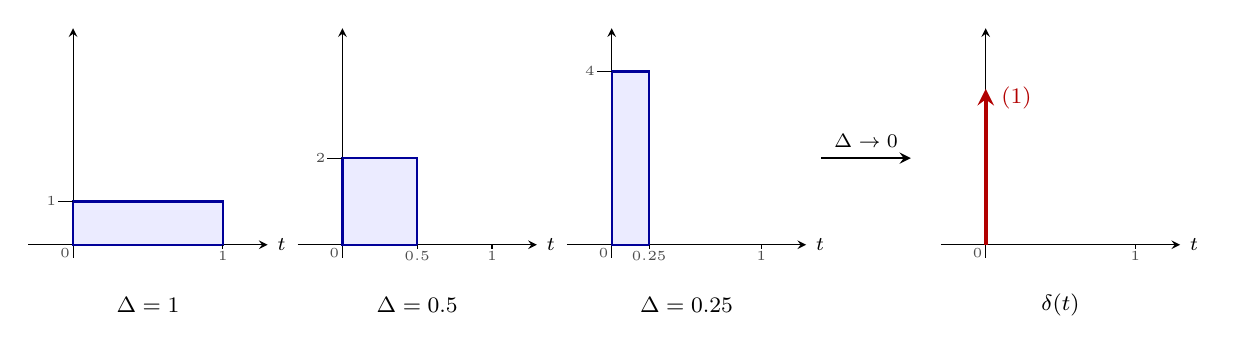
\begin{tikzpicture}[x=1.9cm,y=0.55cm]
  \begin{scope}
    \taxes{-0.3}{1.3}{5.0}
    \draw[sig,fill=blue!8] (0,0) rectangle (1,1);
    \xt{1}{1}\yt{1}{1}
    \node[font=\footnotesize] at (0.5,-1.4) {$\Delta=1$};
  \end{scope}
  \begin{scope}[shift={(1.8,0)}]
    \taxes{-0.3}{1.3}{5.0}
    \draw[sig,fill=blue!8] (0,0) rectangle (0.5,2);
    \xt{0.5}{0.5}\xt{1}{1}\yt{2}{2}
    \node[font=\footnotesize] at (0.5,-1.4) {$\Delta=0.5$};
  \end{scope}
  \begin{scope}[shift={(3.6,0)}]
    \taxes{-0.3}{1.3}{5.0}
    \draw[sig,fill=blue!8] (0,0) rectangle (0.25,4);
    \xt{0.25}{0.25}\xt{1}{1}\yt{4}{4}
    \node[font=\footnotesize] at (0.5,-1.4) {$\Delta=0.25$};
  \end{scope}
  \draw[->,thick] (5.0,2) -- (5.6,2) node[midway,above,font=\scriptsize] {$\Delta\to0$};
  \begin{scope}[shift={(6.1,0)}]
    \taxes{-0.3}{1.3}{5.0}
    \draw[->,ultra thick,red!70!black] (0,0) -- (0,3.6);
    \node[anchor=west,font=\footnotesize,red!70!black] at (0.04,3.4) {$(1)$};
    \xt{1}{1}
    \node[font=\footnotesize] at (0.5,-1.4) {$\delta(t)$};
  \end{scope}
\end{tikzpicture}
\caption{$\delta_\Delta(t)$ 随 $\Delta$ 变小：越来越窄、越来越高，面积始终为 $1$（$1\times1$、$0.5\times2$、$0.25\times4$）。极限就是冲激函数 $\delta(t)$，画成 $t=0$ 处的箭头，标 $(1)$。}
\end{figure}

\subsection{冲激响应}
\begin{itemize}[nosep]
\item 设 $\delta_\Delta(t)$ 通过 LTI 系统的输出为 $h_\Delta(t)$（某个函数）。
\item $\delta(t)=\lim\limits_{\Delta\to0}\delta_\Delta(t)$ 通过同一个 LTI 系统的输出记作 $h(t)$：
\[
h(t)=\lim_{\Delta\to0}h_\Delta(t)\qquad(\text{假设这个极限存在}).
\]
\end{itemize}

\begin{figure}[H]
\centering
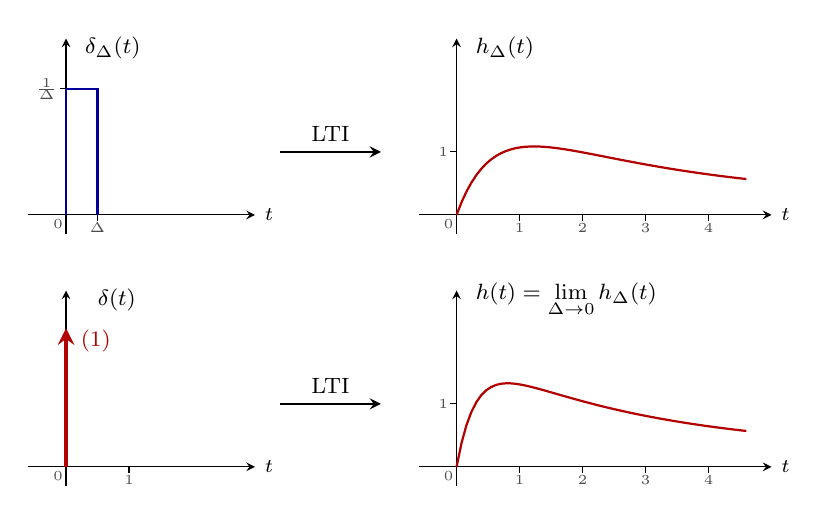
\begin{tikzpicture}[x=0.8cm,y=0.8cm]
  \begin{scope}
    \taxes{-0.6}{3.0}{2.8}
    \draw[sig] (0,0) -- (0,2) -- (0.5,2) -- (0.5,0);
    \xt{0.5}{\Delta}\yt{2}{\frac{1}{\Delta}}
    \node[anchor=west,font=\footnotesize] at (0.15,2.65) {$\delta_\Delta(t)$};
  \end{scope}
  \draw[->,thick] (3.4,1) -- (5.0,1) node[midway,above,font=\footnotesize] {LTI};
  \begin{scope}[shift={(6.2,0)}]
    \taxes{-0.6}{5.0}{2.8}
    \draw[res,domain=0:4.6,samples=60] plot (\x,{1.6*(1-exp(-1.5*\x))*exp(-0.35*\x)+0.25*(1-exp(-1.5*\x))});
    \foreach \p in {1,2,3,4}{\xt{\p}{\p}}\yt{1}{1}
    \node[anchor=west,font=\footnotesize] at (0.15,2.65) {$h_\Delta(t)$};
  \end{scope}
  \begin{scope}[shift={(0,-4.0)}]
    \taxes{-0.6}{3.0}{2.8}
    \draw[->,ultra thick,red!70!black] (0,0) -- (0,2.2);
    \node[anchor=west,font=\footnotesize,red!70!black] at (0.08,2.0) {$(1)$};
    \xt{1}{1}
    \node[anchor=west,font=\footnotesize] at (0.35,2.65) {$\delta(t)$};
    \draw[->,thick] (3.4,1) -- (5.0,1) node[midway,above,font=\footnotesize] {LTI};
    \begin{scope}[shift={(6.2,0)}]
      \taxes{-0.6}{5.0}{2.8}
      \draw[res,domain=0:4.6,samples=60] plot (\x,{1.6*(1-exp(-3*\x))*exp(-0.35*\x)+0.25*(1-exp(-3*\x))});
      \foreach \p in {1,2,3,4}{\xt{\p}{\p}}\yt{1}{1}
      \node[anchor=west,font=\footnotesize] at (0.15,2.65) {$h(t)=\lim\limits_{\Delta\to0}h_\Delta(t)$};
    \end{scope}
  \end{scope}
\end{tikzpicture}
\caption{上：窄方波 $\delta_\Delta(t)$ 的输出 $h_\Delta(t)$。下：$\Delta\to0$ 时输入变成 $\delta(t)$，输出变成 $h(t)$。右边的曲线只是示意形状，具体由系统决定。}
\end{figure}

\begin{remember}
\textbf{冲激响应}(impulse response) $h(t)$：冲激函数 $\delta(t)$ 输入 LTI 系统得到的输出。它对应离散时的单位脉冲响应 $h[n]$。
\end{remember}

%==================================================================
\section{推导连续卷积公式}\label{sec:derive}
思路和离散完全一样：\textbf{拆成窄方波 $\to$ 每个窄方波单独过系统 $\to$ 加起来}；唯一多出的一步是最后令 $\Delta\to0$。

\subsection{\texorpdfstring{第一步：把 $x(t)$ 写成窄方波之和}{第一步：把 x(t) 写成窄方波之和}}
用宽度为 $\Delta$ 的阶梯函数近似 $x(t)$：在 $[k\Delta,(k+1)\Delta)$ 上取高度 $x(k\Delta)$（左端点处 $x(t)$ 的值）。把这条红色阶梯函数记作 $x_\Delta(t)$：

\begin{remember}
\[
x_\Delta(t)=\sum_{k=-\infty}^{+\infty}x(k\Delta)\,\delta_\Delta(t-k\Delta)\cdot\Delta .
\]
这是整个推导中\textbf{最难理解的一步}，下面逐块解释。
\end{remember}

\begin{figure}[H]
\centering
\begin{tikzpicture}[x=1.15cm,y=1.1cm]
  \taxes{-2.7}{4.4}{2.7}
  \draw[thick,gray!60!black,domain=-2.5:4.0,samples=80] plot (\x,{xf(\x)});
  \foreach \a in {-2,-1,3}{%
    \pgfmathsetmacro{\h}{xf(\a)}
    \draw[red!70!black,thick,fill=red!10] (\a,0) rectangle ({\a+1},\h);}
  \pgfmathsetmacro{\ha}{xf(0)}\pgfmathsetmacro{\hb}{xf(1)}\pgfmathsetmacro{\hc}{xf(2)}
  \draw[red!70!black,thick,fill=blue!25] (0,0) rectangle (1,\ha);
  \draw[red!70!black,thick,fill=violet!25] (1,0) rectangle (2,\hb);
  \draw[red!70!black,thick,fill=green!25] (2,0) rectangle (3,\hc);
  \node[font=\scriptsize,anchor=north] at (0.5,{\ha-0.1}) {$x(0)$};
  \node[font=\scriptsize,anchor=north] at (1.5,{\hb-0.1}) {$x(\Delta)$};
  \node[font=\scriptsize,anchor=north] at (2.5,{\hc-0.1}) {$x(2\Delta)$};
  \xt{-2}{-2\Delta}\xt{-1}{-\Delta}\xt{1}{\Delta}\xt{2}{2\Delta}\xt{3}{3\Delta}\xt{4}{4\Delta}
  \yt{1}{1}\yt{2}{2}
\end{tikzpicture}
\caption{阶梯函数 $x_\Delta(t)$ （红色）由一块块宽为 $\Delta$ 的矩形拼成，灰色曲线是 $x(t)$。蓝、紫、绿三块分别对应 $k=0,1,2$，高度是左端点处的 $x(0)$、$x(\Delta)$、$x(2\Delta)$。}
\end{figure}

\point{蓝色块（$k=0$）。}它从 $0$ 到 $\Delta$，高度 $x(0)$，等于
\[
x(0)\,\delta_\Delta(t)\cdot\Delta .
\]
原因：$\delta_\Delta(t)$ 是 $0$ 到 $\Delta$ 的方波，高度 $\frac1\Delta$；乘 $\Delta$ 后高度变成 $1$；再乘 $x(0)$，高度变成 $x(0)$。

\point{紫色块（$k=1$）。}它从 $\Delta$ 到 $2\Delta$，高度 $x(\Delta)$，等于
\[
x(\Delta)\,\delta_\Delta(t-\Delta)\cdot\Delta .
\]
$\delta_\Delta(t-\Delta)$ 是把 $0$ 到 $\Delta$ 的方波右移 $\Delta$，变成 $\Delta$ 到 $2\Delta$ 的方波；乘 $\Delta$ 的作用和蓝色块一样，把高度 $\frac1\Delta$ 变成 $1$，再由 $x(\Delta)$ 定高度。

\point{绿色块（$k=2$）。}从 $2\Delta$ 到 $3\Delta$，高度 $x(2\Delta)$，等于 $x(2\Delta)\,\delta_\Delta(t-2\Delta)\cdot\Delta$：方波右移 $2\Delta$。

以此类推，第 $k$ 块是 $x(k\Delta)\,\delta_\Delta(t-k\Delta)\cdot\Delta$，把所有块加起来就是上面的公式。

\begin{figure}[H]
\centering
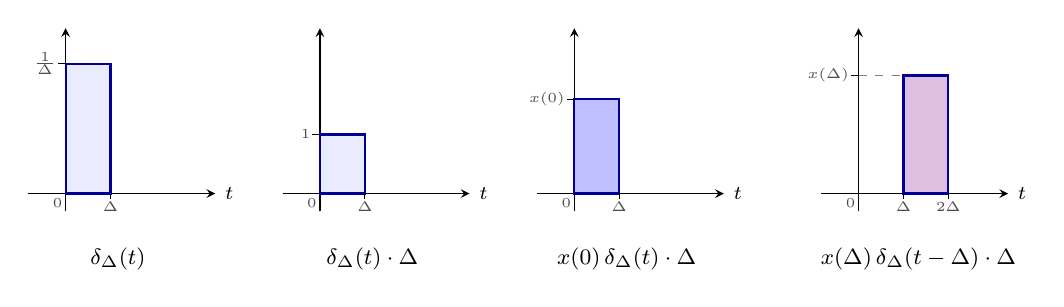
\begin{tikzpicture}[x=0.95cm,y=0.75cm]
  \begin{scope}
    \taxes{-0.5}{2.0}{2.8}
    \draw[sig,fill=blue!8] (0,0) rectangle (0.6,2.2);
    \xt{0.6}{\Delta}\yt{2.2}{\frac{1}{\Delta}}
    \node[font=\footnotesize] at (0.7,-1.1) {$\delta_\Delta(t)$};
  \end{scope}
  \begin{scope}[shift={(3.4,0)}]
    \taxes{-0.5}{2.0}{2.8}
    \draw[sig,fill=blue!8] (0,0) rectangle (0.6,1);
    \xt{0.6}{\Delta}\yt{1}{1}
    \node[font=\footnotesize] at (0.7,-1.1) {$\delta_\Delta(t)\cdot\Delta$};
  \end{scope}
  \begin{scope}[shift={(6.8,0)}]
    \taxes{-0.5}{2.0}{2.8}
    \draw[sig,fill=blue!25] (0,0) rectangle (0.6,1.6);
    \xt{0.6}{\Delta}\yt{1.6}{x(0)}
    \node[font=\footnotesize] at (0.7,-1.1) {$x(0)\,\delta_\Delta(t)\cdot\Delta$};
  \end{scope}
  \begin{scope}[shift={(10.6,0)}]
    \taxes{-0.5}{2.0}{2.8}
    \draw[sig,fill=violet!25] (0.6,0) rectangle (1.2,2.0);
    \xt{0.6}{\Delta}\xt{1.2}{2\Delta}\yt{2.0}{x(\Delta)}
    \draw[dashed,gray] (0,2.0) -- (0.6,2.0);
    \node[font=\footnotesize] at (0.8,-1.1) {$x(\Delta)\,\delta_\Delta(t-\Delta)\cdot\Delta$};
  \end{scope}
\end{tikzpicture}
\caption{一块矩形是怎么来的：$\delta_\Delta(t)$ 高 $\frac1\Delta$，乘 $\Delta$ 后高 $1$，再乘 $x(0)$ 后高 $x(0)$（蓝色块）。把方波右移 $\Delta$、乘 $x(\Delta)$，得到紫色块。}
\end{figure}

\point{取极限。}$\Delta$ 取得特别小时，阶梯函数与 $x(t)$ 保持一致：
\[
\lim_{\Delta\to0}x_\Delta(t)=x(t).
\]

\subsection{第二步：逐条性质推出输出}
\needspace{12\baselineskip}
\begin{center}
\renewcommand{\arraystretch}{1.5}
\begin{tabular}{@{}p{4.3cm}p{4.3cm}p{6.3cm}@{}}
\toprule
输入 & 输出 & 依据\\
\midrule
$\delta_\Delta(t)$ & $h_\Delta(t)$ & $h_\Delta(t)$ 的定义\\
$\delta_\Delta(t-k\Delta)$ & $h_\Delta(t-k\Delta)$ & \textbf{时不变性}：输入右移 $k\Delta$，输出也右移 $k\Delta$\\
$x(k\Delta)\,\delta_\Delta(t-k\Delta)\cdot\Delta$ & $x(k\Delta)\,h_\Delta(t-k\Delta)\cdot\Delta$ & \textbf{齐次性}：系数 $a=x(k\Delta)\cdot\Delta$\\
$\displaystyle\sum_{k=-\infty}^{+\infty}x(k\Delta)\,\delta_\Delta(t-k\Delta)\cdot\Delta$ & $\displaystyle\sum_{k=-\infty}^{+\infty}x(k\Delta)\,h_\Delta(t-k\Delta)\cdot\Delta$ & \textbf{叠加性}：输入全部加起来，输出也全部加起来\\
\bottomrule
\end{tabular}
\end{center}
最后一行左边就是 $x_\Delta(t)$（第一步）。所以阶梯函数 $x_\Delta(t)$ 的输出是 $\sum_k x(k\Delta)\,h_\Delta(t-k\Delta)\cdot\Delta$。

\subsection{\texorpdfstring{第三步：令 $\Delta\to0$，求和变成积分}{第三步：令 Δ→0，求和变成积分}}
两边同时令 $\Delta\to0$。左边 $\lim x_\Delta(t)=x(t)$，所以 $x(t)$ 通过 LTI 的输出 $y(t)$ 为
\begin{align*}
y(t)&=\lim_{\Delta\to0}\sum_{k=-\infty}^{+\infty}x(k\Delta)\,h_\Delta(t-k\Delta)\cdot\Delta\\[2pt]
&=\lim_{\Delta\to0}\sum_{k=-\infty}^{+\infty}x(k\Delta)\,h(t-k\Delta)\cdot\Delta
&&\text{（$\Delta\to0$ 时 $h_\Delta\to h$）}\\[2pt]
&=\int_{-\infty}^{+\infty}x(\tau)\,h(t-\tau)\,\mathrm{d}\tau
&&\text{（黎曼积分的定义）}
\end{align*}

\point{第二个等号。}$h_\Delta$ 换成 $h$，因为 $\Delta\to0$ 时 $h_\Delta(t)$ 趋于 $h(t)$（冲激响应的定义）。

\point{第三个等号。}这就是积分的定义（黎曼和取极限）：

\begin{center}
\begin{tabular}{@{}lll@{}}
\toprule
求和里的 & 积分里的 & 含义\\
\midrule
$k\Delta$ & $\tau$ & 第 $k$ 块所在的位置\\
$\Delta$ & $\mathrm{d}\tau$ & 每块的宽度\\
$\displaystyle\lim_{\Delta\to0}\sum_{k=-\infty}^{+\infty}$ & $\displaystyle\int_{-\infty}^{+\infty}$ & 把所有块加起来\\
\bottomrule
\end{tabular}
\end{center}

\begin{note}
推导中有两处默认成立：一是 $h(t)=\lim_{\Delta\to0}h_\Delta(t)$ 这个极限存在；二是输入取极限（$x_\Delta\to x$）时，输出也取对应的极限。对后面遇到的系统，这两点都成立。
\end{note}

\subsection{结论：卷积积分}
\begin{remember}
若 $\delta(t)\xrightarrow{\ \text{LTI}\ }h(t)$，则任意 $x(t)$ 通过同一个 LTI，输出为
\[
y(t)=x(t)\ast h(t)=\int_{-\infty}^{+\infty}x(\tau)\,h(t-\tau)\,\mathrm{d}\tau\qquad(\text{教材第 38 页式 2-11、2-12}).
\]
\begin{itemize}[nosep]
\item $\delta(t)$：冲激函数；$h(t)$：冲激响应。
\item 这个公式定义为 $x(t)$ 与 $h(t)$ 的\textbf{卷积}(convolution)，记作 $x(t)\ast h(t)$。
\item 和离散一样：\textbf{只要知道 $h(t)$，就能求出任意输入的输出}。
\end{itemize}
\end{remember}

%==================================================================
\section{离散卷积与连续卷积；「卷积」名字的由来}\label{sec:name}
\subsection{两个公式对照}
\begin{remember}
\begin{align*}
\text{离散卷积：}\quad x[n]\ast h[n]&=\sum_{k=-\infty}^{+\infty}x[k]\,h[n-k],\\
\text{连续卷积：}\quad x(t)\ast h(t)&=\int_{-\infty}^{+\infty}x(\tau)\,h(t-\tau)\,\mathrm{d}\tau .
\end{align*}
这两个公式要能倒背如流。
\end{remember}

\begin{center}
\begin{tabular}{@{}lll@{}}
\toprule
 & 离散 & 连续\\
\midrule
基本输入 & 单位脉冲 $\delta[n]$ & 冲激函数 $\delta(t)$\\
它的输出 & 单位脉冲响应 $h[n]$ & 冲激响应 $h(t)$\\
求和变量 & $k$（整数） & $\tau$（实数）\\
合成方式 & 求和 $\sum$ & 积分 $\int\cdots\mathrm{d}\tau$\\
推导方式 & 拆成脉冲，直接相加，结果精确 & 拆成窄方波，相加后再令 $\Delta\to0$\\
\bottomrule
\end{tabular}
\end{center}

\subsection{卷积的四步与名字}
把 $h(t-\tau)$ 写成 $h[-(\tau-t)]$：
\[
x(t)\ast h(t)=\int_{-\infty}^{+\infty}x(\tau)\,h\big[-(\tau-t)\big]\,\mathrm{d}\tau .
\]
从里往外读，正好是卷积的四步：
\begin{enumerate}[nosep]
\item \textbf{翻转}：$h(\tau)\to h(-\tau)$，沿纵轴翻过来；
\item \textbf{平移}：$h(-\tau)\to h[-(\tau-t)]$，平移 $t$；
\item \textbf{相乘}：与 $x(\tau)$ 相乘；
\item \textbf{积分}（离散时是\textbf{求和}）：对 $\tau$ 积分，得到 $y(t)$ 在这一个 $t$ 上的值。
\end{enumerate}

\begin{figure}[H]
\centering
\begin{tikzpicture}[x=0.85cm,y=1.3cm]
  \begin{scope}
    \taxes[\tau]{-2.6}{2.8}{1.6}
    \draw[res] (0,0) -- (0,1) -- (2,0);
    \foreach \p in {-2,-1,1,2}{\xt{\p}{\p}}\yt{1}{1}
    \node[anchor=west,font=\footnotesize] at (0.15,1.5) {(1) $h(\tau)$};
  \end{scope}
  \begin{scope}[shift={(7.2,0)}]
    \taxes[\tau]{-2.6}{2.8}{1.6}
    \draw[res] (-2,0) -- (0,1) -- (0,0);
    \foreach \p in {-2,-1,1,2}{\xt{\p}{\p}}
    \draw (0,1) -- (0.1,1) node[anchor=west,font=\tiny,gray!60!black,fill=white,inner sep=0.6pt] {$1$};
    \node[anchor=west,font=\footnotesize] at (0.15,1.5) {(2) 翻转：$h(-\tau)$};
  \end{scope}
  \begin{scope}[shift={(0,-2.4)}]
    \taxes[\tau]{-2.6}{2.8}{1.6}
    \draw[res] (-1,0) -- (1,1) -- (1,0);
    \foreach \p in {-2,-1,1,2}{\xt{\p}{\p}}\yt{1}{1}
    \node[anchor=west,font=\footnotesize] at (0.15,1.5) {(3) 平移 $t=1$：$h(1-\tau)$};
  \end{scope}
  \begin{scope}[shift={(7.2,-2.4)}]
    \taxes[\tau]{-2.6}{2.8}{1.6}
    \fill[orange!35] (0,0) -- (0,0.5) -- (1,1) -- (1,0) -- cycle;
    \draw[sig,dashed] (0,0) -- (0,1) -- (2,1) -- (2,0);
    \draw[res] (-1,0) -- (1,1) -- (1,0);
    \foreach \p in {-2,-1,1,2}{\xt{\p}{\p}}\yt{1}{1}
    \node[anchor=west,font=\footnotesize] at (0.15,1.5) {(4) 乘 $x(\tau)$ 再积分};
  \end{scope}
\end{tikzpicture}
\caption{以 $h(\tau)$ 为 $[0,2]$ 上从 $1$ 降到 $0$ 的斜线、$x(\tau)$ 为 $[0,2]$ 上高度 $1$ 的方波（图 (4) 中蓝虚线）为例求 $y(1)$。翻转、平移后 $h(1-\tau)$ 在 $[-1,1]$ 上，与 $x(\tau)$ 重叠在 $[0,1]$，乘积从 $0.5$ 升到 $1$，橙色面积 $=\frac{0.5+1}{2}\times1=0.75$，即 $y(1)=0.75$。}
\end{figure}

\begin{remember}
\textbf{卷积}(convolution)的名字取自四步中的两步：\textbf{「卷」指翻转，「积」指相乘}。
\end{remember}

\end{document}
